%----------------------------------------------------------------------------------------
% METADATA BLOCK (YAML)  — see inbox/README.md
%----------------------------------------------------------------------------------------
% uid: ""
% school: "lycee"
% level: "2eme"
% section: ["Sciences", "Informatique"]
% chapter: "Barycentre"
% title: "Synthèse : ensembles de points dans un rectangle"
% difficulty: "Moyen"
% tags: ["barycentre", "ensemble-de-points", "cercle", "mediatrice"]
% provenance: "own"
% batch: "2026-11-19-2sc-polynomes-barycentre"
%----------------------------------------------------------------------------------------

\newcommand{\R}{\mathbb{R}}
\newcommand{\vect}[1]{\overrightarrow{#1}}

% ---STATEMENT---
Soit $ABCD$ un rectangle tel que $AB=6$ cm et $AD=4$ cm. On note $I$ le milieu de $[AB]$ et $J$ le milieu de $[CD]$.
\begin{enumerate}
  \item Montrer que $D$ est le barycentre de $(A,1)$, $(B,-1)$ et $(C,1)$.
  \item Déterminer et construire l'ensemble $E_1$ des points $M$ tels que $\bigl\|\vect{MA}+\vect{MB}\bigr\|=\bigl\|\vect{MC}+\vect{MD}\bigr\|$.
  \item Soit $G$ le barycentre de $(A,1)$, $(B,1)$ et $(C,2)$.
  \begin{enumerate}
    \item Montrer que $G$ est le milieu de $[IC]$ et que $G\in E_1$.
    \item Déterminer et construire l'ensemble $E_2$ des points $M$ tels que $\bigl\|\vect{MA}+\vect{MB}+2\vect{MC}\bigr\|=8$.
    \item Construire les points communs à $E_1$ et $E_2$.
  \end{enumerate}
  \item Déterminer l'ensemble $E_3$ des points $M$ tels que $\bigl\|\vect{MA}-\vect{MB}+\vect{MC}\bigr\|=AC$. Vérifier que $B\in E_3$.
\end{enumerate}

% ---SOLUTION---
\begin{center}
% alt: Rectangle ABCD, I et J milieux de [AB] et [CD], droite E1 à mi-hauteur, cercle E2 de centre G, grand cercle E3 de centre D passant par B.
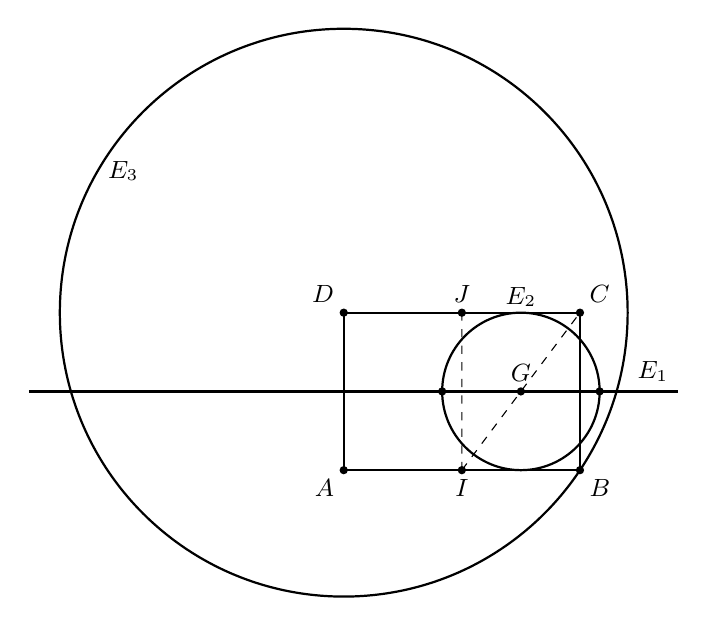
\begin{tikzpicture}[scale=0.5, font=\small]
  \coordinate (A) at (0,0); \coordinate (B) at (6,0); \coordinate (C) at (6,4); \coordinate (D) at (0,4);
  \coordinate (I) at (3,0); \coordinate (J) at (3,4); \coordinate (G) at (4.5,2);
  \draw[black, thick] (D) circle (7.2111);
  \draw[thick] (G) circle (2);
  \draw[thick] (A)--(B)--(C)--(D)--cycle;
  \draw[dashed] (I)--(C) (I)--(J);
  \draw[black, thick] (-8,2)--(8.5,2) node[above left, text=black] {$E_1$};
  \foreach \p/\pos in {A/below left, B/below right, C/above right, D/above left, I/below, J/above, G/above}
    \fill (\p) circle (3pt) node[\pos] {$\p$};
  \fill (2.5,2) circle (3pt) (6.5,2) circle (3pt);
  \node[text=black] at (4.5,4.4) {$E_2$};
  \node[text=black] at (-5.6,7.6) {$E_3$};
\end{tikzpicture}
\end{center}
\begin{enumerate}[itemsep=14pt]
  \item
  \begin{prop}[Parallélogramme]
  $ABCD$ est un parallélogramme si et seulement si \ib{$\vect{DA}+\vect{DC}=\vect{DB}$}.
  \end{prop}
  Un rectangle est un parallélogramme, donc :
  \[\vect{DA}-\vect{DB}+\vect{DC}=\vect{DB}-\vect{DB}=\vec0\]
  La somme $1-1+1=1\neq0$ : $D$ est le barycentre de $(A,1)$, $(B,-1)$, $(C,1)$.

  \item
  \begin{prop}[Milieu]
  Si $I$ est le milieu de $[AB]$ : \ib{$\vect{MA}+\vect{MB}=2\vect{MI}$} pour tout point $M$.
  \end{prop}
  De même $\vect{MC}+\vect{MD}=2\vect{MJ}$. La condition devient
  \[2MI=2MJ\iff MI=MJ\]
  $E_1$ est la \textbf{médiatrice de $[IJ]$} : la droite parallèle à $(AB)$ qui passe par les milieux de $[AD]$ et de $[BC]$.

  \item
  \begin{enumerate}[itemsep=10pt]
    \item On remplace $(A,1)$ et $(B,1)$ par leur barycentre $(I,2)$ : $G$ est le barycentre de $(I,2)$ et $(C,2)$, c'est le milieu de $[IC]$.

    Pour montrer que $G\in E_1$, on se place dans le repère orthonormé d'origine $A$, d'unité $1$ cm, avec $B(6\,;0)$ et $D(0\,;4)$ :
    \[I(3\,;0)\qquad J(3\,;4)\qquad C(6\,;4)\qquad G\left(\dfrac{3+6}{2}\,;\dfrac{0+4}{2}\right)=\left(\dfrac92\,;2\right)\]
    La médiatrice de $[IJ]$ est la droite d'équation $y=2$ ; comme $y_G=2$, on a bien $G\in E_1$.

    \item
    \begin{prop}[Réduction d'une somme vectorielle]
    Si $\alpha+\beta+\gamma\neq0$ et $G$ est le barycentre de $(A,\alpha),(B,\beta),(C,\gamma)$ :
    \ib{$\alpha\vect{MA}+\beta\vect{MB}+\gamma\vect{MC}=(\alpha+\beta+\gamma)\vect{MG}$}.
    \end{prop}
    Ici $1+1+2=4$ : la condition devient $4MG=8$, soit $MG=2$.

    $E_2$ est le \textbf{cercle de centre $G$ et de rayon $2$ cm}.

    \item $G$ est sur la droite $E_1$ : la droite coupe le cercle $E_2$ en deux points, situés sur $E_1$ à $2$ cm de part et d'autre de $G$, c'est-à-dire $\left(\dfrac52\,;2\right)$ et $\left(\dfrac{13}{2}\,;2\right)$ dans le repère précédent.
  \end{enumerate}

  \item D'après 1), la somme vaut $1$ et $\vect{MA}-\vect{MB}+\vect{MC}=\vect{MD}$. La condition devient $MD=AC$.

  $E_3$ est le \textbf{cercle de centre $D$ et de rayon $AC$}, avec $AC=\sqrt{6^2+4^2}=\sqrt{52}=2\sqrt{13}$ cm.

  Les diagonales d'un rectangle ont la même longueur : $DB=AC$, donc $B\in E_3$.
\end{enumerate}
\textbf{Idée :} chaque somme se réduit à un seul vecteur $k\vect{MP}$ ; on obtient une médiatrice ($MP=MQ$) ou un cercle ($MP=r$).

\textbf{Piège :} pour $E_3$, le barycentre est le sommet $D$ lui-même, que l'on reconnaît grâce au parallélogramme.
